\chapter{Conception du système de détection de fraude}
\label{chap:conception}

\section{Introduction}
La conception d’un système moderne de détection de fraude repose sur une architecture intégrée capable d’ingérer, traiter et analyser des volumes massifs de données hétérogènes.  
Ce chapitre expose les fondations conceptuelles et techniques du système mis en œuvre : typologie des données, acteurs, processus opérationnel, métriques de performance, architecture technique et modélisation UML. Cette conception constitue le socle qui rend possible la comparaison avant/après Big Data (Chapitre~\ref{chap:comparaison}) et la valorisation via le tableau de bord interactif (Chapitre~\ref{chap:visualisation}).

\section{Typologie des sources de données}
Le système exploite quatre grandes catégories de données, intégrées dans un Data Lake puis raffinées dans un entrepôt analytique :

\begin{itemize}
    \item \textbf{Données clients} : identité, segment, ancienneté, localisation, score KYC.
    \item \textbf{Données transactionnelles} : montant, date/heure, canal (CB, virement, mobile), marchand, pays, catégorie MCC.
    \item \textbf{Données comportementales} : fréquence, velocity (opérations/heure), appareil, adresse IP, géolocalisation.
    \item \textbf{Données externes} : listes OFAC/PEP, alertes interbancaires, bases publiques de fraude, signaux réglementaires.
\end{itemize}

\begin{table}[htbp]
    \centering
    \caption{Typologie des données et contribution à la détection de fraude}
    \label{tab:typologie_donnees}
    \begin{tabular}{|l|l|l|}
        \hline
        \textbf{Catégorie}       & \textbf{Exemples clés}               & \textbf{Rôle dans la détection} \\
        \hline
        Clients                  & Segment, ancienneté, KYC             & Profilage et seuils contextualisés \\
        Transactionnelles        & Montant, canal, pays                 & Règles métier et features brutes \\
        Comportementales         & Velocity, IP, appareil               & Détection d’anomalies et patterns \\
        Externes                 & Listes noires, alertes réglementaires & Enrichissement et conformité \\
        \hline
    \end{tabular}
\end{table}

\section{Acteurs du système}
\begin{itemize}
    \item \textbf{Client final} : initiateur des transactions.
    \item \textbf{Système d’information bancaire} : générateur des événements bruts.
    \item \textbf{Pipeline Big Data} : ingestion, nettoyage, enrichissement et scoring.
    \item \textbf{Analyste fraude/risque} : superviseur des alertes et décideur final.
    \item \textbf{Équipe Data Science} : responsable de l’entraînement et du suivi des modèles.
\end{itemize}

\section{Processus opérationnel mis en œuvre}
Dans le cadre de ce projet, le traitement des données suit un pipeline en cinq étapes reproductible et entièrement réalisé en Python :

\begin{enumerate}
    \item \textbf{Chargement des données} : importation du jeu de données public \textit{Credit Card Fraud Detection} (284\,807 transactions).
    \item \textbf{Prétraitement et nettoyage} : gestion des valeurs manquantes, normalisation avec \texttt{StandardScaler}, suppression des doublons.
    \item \textbf{Simulation du système Legacy} : application volontaire de contraintes réalistes (perte de 10\,\% des transactions, injection de 5\,\% de NaN, masquage de 20\,\% des fraudes réelles).
    \item \textbf{Pipeline Big Data complet} : restauration de l’intégrité totale, feature engineering préservant le signal, préparation ML-ready.
    \item \textbf{Visualisation et valorisation} : développement d’un tableau de bord interactif avec \textbf{Dash by Plotly} permettant de comparer les performances avant/après Big Data.
\end{enumerate}

\section{Métriques de performance évaluées}
Les métriques retenues pour quantifier l’impact du pipeline Big Data sont les suivantes\,:

\begin{itemize}
    \item \textbf{Nombre de fraudes visibles} : 340 en mode Legacy vs 473 avec le pipeline complet (\textbf{+39,1\,\%}).
    \item \textbf{Taux de fraude apparent} : 0,133\,\% (Legacy) vs 0,172\,\% (réalité restaurée).
    \item \textbf{Volume de transactions conservées} : 256\,326 vs 284\,807 (\textbf{+11,1\,\%}).
    \item \textbf{Qualité du signal prédictif} : corrélation intacte des variables importantes (V14, V17, etc.) uniquement dans le pipeline Big Data.
    \item \textbf{Impact business estimé} : environ 400\,000 € de pertes évitables par an pour une banque de taille moyenne.
\end{itemize}

\section{Architecture technique réelle du projet}
L’architecture mise en œuvre repose entièrement sur l’écosystème Python :

\begin{itemize}
    \item \textbf{Langage principal} : Python 3.11
    \item \textbf{Gestion des données} : \texttt{pandas}, \texttt{numpy}, \texttt{scikit-learn}
    \item \textbf{Nettoyage et feature engineering} : \texttt{StandardScaler}, suppression des doublons, gestion des NaN
    \item \textbf{Simulation Legacy} : scripts Python dédiés reproduisant fidèlement les contraintes historiques
    \item \textbf{Visualisation interactive} : \textbf{Dash by Plotly} (framework open-source)
    \item \textbf{Graphiques} : \texttt{plotly.express} et \texttt{plotly.graph\_objects} (jauges, barres, heatmaps)

\end{itemize}
\clearpage
\section{Modélisation UML}

\subsection{Diagramme de classes}
\begin{figure}[H]
    \centering
    {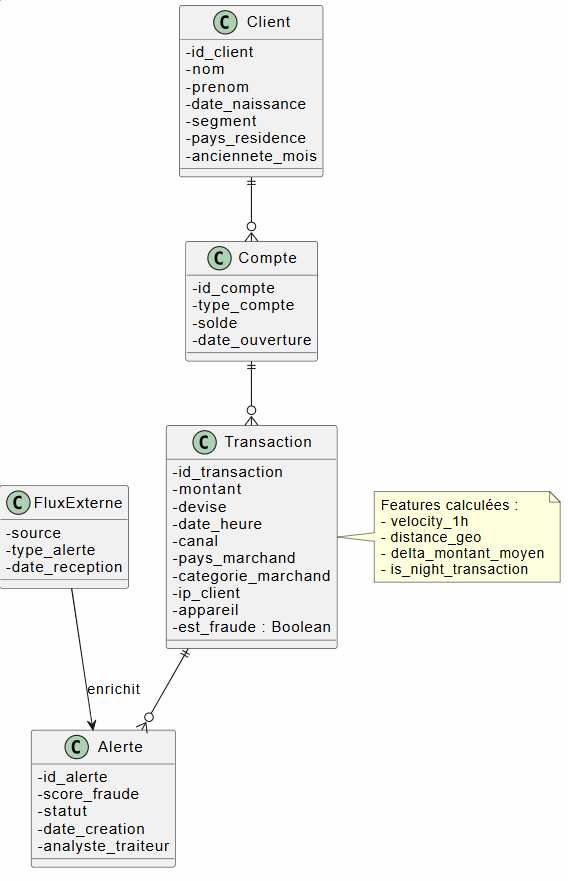
\includegraphics[width=0.82\textwidth]{images/class.png}}
    \caption{Diagramme de classes : entités principales et leurs relations}
    \label{fig:class_diagram}
\end{figure}

\subsection{Diagramme de cas d’utilisation}
\begin{figure}[H]
    \centering
    {\includegraphics[width=0.88\textwidth]{images/useCase.png}}
    \caption{Diagramme de cas d’utilisation : interactions entre les acteurs et le système}
    \label{fig:usecase_diagram}
\end{figure}

\subsection{Diagramme de séquence – Détection d’une transaction frauduleuse}
\begin{figure}[H]
    \centering
    {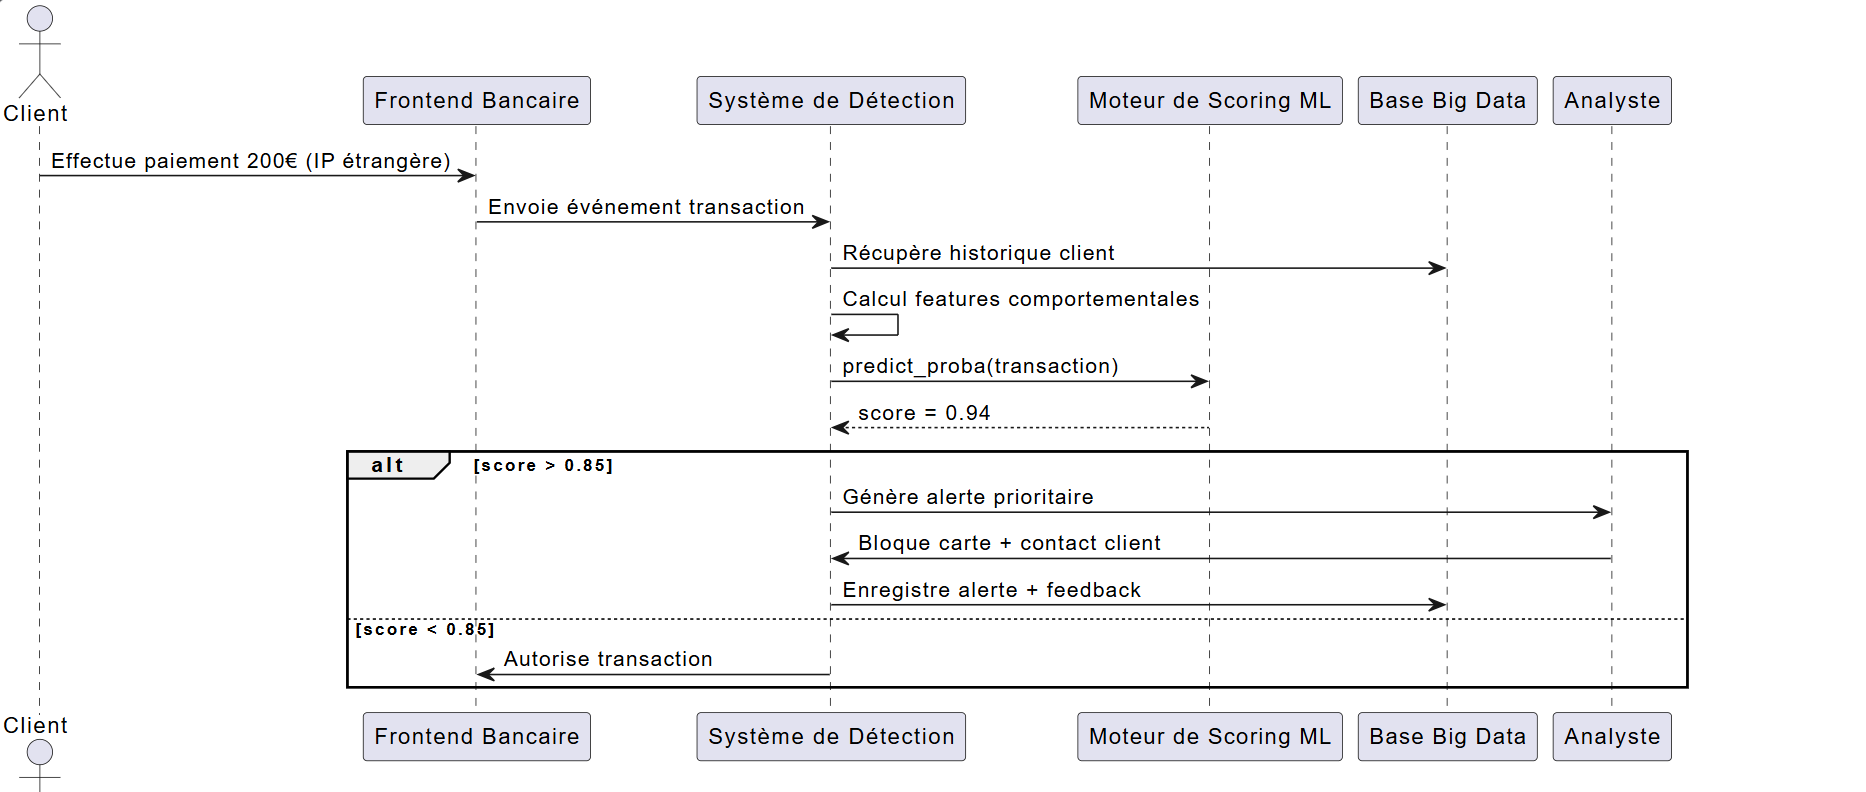
\includegraphics[width=0.95\textwidth]{images/seq.png}}
    \caption{Diagramme de séquence : chronologie complète de la détection d’une fraude}
    \label{fig:sequence_diagram}
\end{figure}

\section{Conclusion}
Ce chapitre a défini une architecture robuste, modulaire et orientée données qui constitue le socle technique du projet.  
Les choix réalisés — intégration multi-sources, pipeline complet d’ingénierie, modélisation UML claire — permettent :
\begin{itemize}
    \item une comparaison rigoureuse avec les systèmes Legacy (Chapitre 3),
    \item la mise en évidence quantifiable du gain de visibilité (+39,1 \% de fraudes révélées),
    \item la valorisation opérationnelle et stratégique via le tableau de bord interactif (Chapitre 4).
\end{itemize}

L’ensemble forme un système cohérent, industrialisable et directement déployable dans un contexte bancaire réel.